\documentclass[11pt, letterpaper]{article}
\usepackage[utf8]{inputenc}
\usepackage[margin=1in]{geometry}
\usepackage{amsmath, amssymb}
\usepackage{booktabs}
\usepackage{float}
\usepackage{graphicx}
\usepackage{tikz}
\usetikzlibrary{arrows.meta}
\usepackage{algorithm}
\usepackage{algorithmic}
\setlength{\parindent}{0pt}
\setlength{\parskip}{0.5em}

% ---------- Packages ----------
\usepackage[margin=1in]{geometry}
\usepackage{amsmath, amssymb, amsthm}
\usepackage{enumitem}
\usepackage{graphicx}
\usepackage{xcolor}
\usepackage{tcolorbox}
\usepackage{hyperref}
\usepackage{float}
\usepackage{booktabs}
\usepackage{parskip}

% ---------- Basic Info ----------
\title{CSC311 final project ML}
\author{Meixuan Lou}
\date{July 2026}

% ---------- Question Box ----------
\newtcolorbox{questionbox}{
  colback=gray!8,
  colframe=gray!60,
  boxrule=0.5pt,
  arc=2pt,
  left=6pt,
  right=6pt,
  top=6pt,
  bottom=6pt
}

% ---------- Solution Label ----------
\newcommand{\solution}{\vspace{0.5em}\noindent\textbf{Solution.}\ }

\begin{document}
\begin{center}
    {\LARGE \textbf{CSC311 Summer 2026}} \\[0.5em]
    {\large \textbf{Final Project}} \\[0.5em]
    {\normalsize Xiaohan Ma, Meixuan Lou, Siyi Chen} \\
    {\normalsize Due: Friday, August 7, 2026 before 11:00pm EST}
\end{center}
\vspace{1em}

\section*{Part A}
 
% ============================================================
\subsection*{1. k-Nearest Neighbors}

\subsubsection*{(a) User-based collaborative filtering}

In user-based collaborative filtering, each row represents a student and each column represents a question. KNN identifies students with similar response patterns and uses their answers to estimate missing entries.

We evaluated
\[
k \in \{1,6,11,16,21,26\}.
\]

\begin{table}[H]
    \centering
    \begin{tabular}{cc}
        \toprule
        $k$ & Validation Accuracy \\
        \midrule
        1  & 0.6245 \\
        6  & 0.6781 \\
        11 & 0.6897 \\
        16 & 0.6753 \\
        21 & 0.6681 \\
        26 & 0.6503 \\
        \bottomrule
    \end{tabular}
    \caption{User-based KNN validation accuracy.}
    \label{tab:user_knn}
\end{table}

\begin{figure}[H]
    \centering
    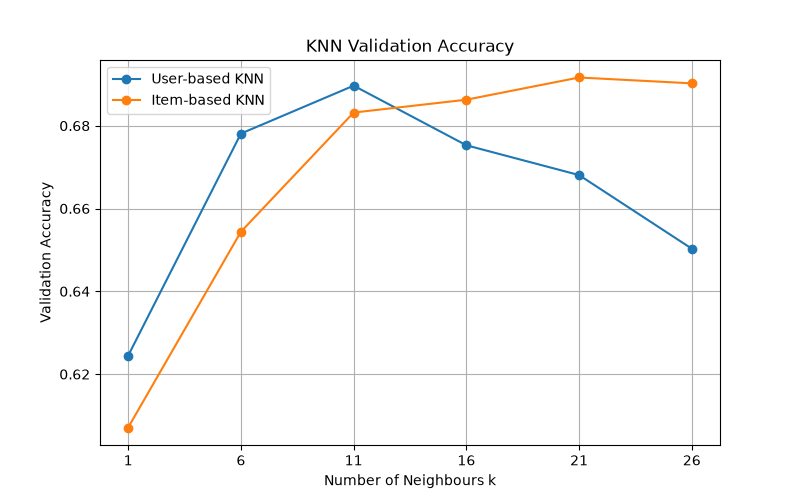
\includegraphics[width=0.65\textwidth]{knn_validation_accuracy.png}
    \caption{Validation accuracy as a function of $k$ for user-based and item-based KNN.}
    \label{fig:knn_validation}
\end{figure}

The validation accuracy increased until $k=11$ and then decreased. A small $k$ can be sensitive to noisy neighbours, while a large $k$ may include less similar students.

\subsubsection*{(b) Selected user-based model}

The highest validation accuracy was $0.6897$ at
\[
k^*_{\text{user}}=11.
\]
Using this value, the test accuracy was
\[
\boxed{0.6847}.
\]

\subsubsection*{(c) Item-based collaborative filtering}

For item-based collaborative filtering, the matrix was transposed so that each row represented a question. KNN then compared questions based on how similarly they were answered by students. The imputed matrix was transposed back before evaluation.

The underlying assumption is that questions with similar response patterns are related, so a student's response to one question can help predict their response to another similar question.

\begin{table}[H]
    \centering
    \begin{tabular}{cc}
        \toprule
        $k$ & Validation Accuracy \\
        \midrule
        1  & 0.6071 \\
        6  & 0.6544 \\
        11 & 0.6832 \\
        16 & 0.6863 \\
        21 & 0.6916 \\
        26 & 0.6902 \\
        \bottomrule
    \end{tabular}
    \caption{Item-based KNN validation accuracy.}
    \label{tab:item_knn}
\end{table}

The highest validation accuracy was $0.6916$ at
\[
k^*_{\text{item}}=21.
\]
Using this value, the test accuracy was
\[
\boxed{0.6828}.
\]

\subsubsection*{(d) Comparison}

\begin{table}[H]
    \centering
    \begin{tabular}{lccc}
        \toprule
        Method & Selected $k$ & Validation Accuracy & Test Accuracy \\
        \midrule
        User-based KNN & 11 & 0.6897 & 0.6847 \\
        Item-based KNN & 21 & 0.6916 & 0.6828 \\
        \bottomrule
    \end{tabular}
    \caption{Comparison of user-based and item-based KNN.}
    \label{tab:knn_comparison}
\end{table}

User-based KNN achieved a slightly higher test accuracy than item-based KNN, although the performances were very similar.

\subsubsection*{(e) Limitations}

One limitation is that the response matrix contains many missing entries. Therefore, the distance between two students or questions may be calculated from only a small amount of shared information and may not reflect true similarity.

A second limitation is that new students or questions have very little response data, making it difficult to identify reliable neighbours.

KNN also does not directly model student ability or question difficulty, and its computational cost increases as the number of students and questions grows.
 
% ============================================================
\subsection*{2. Item Response Theory}
 
\subsubsection*{(a) Derivation}
 
Let $C \in \{0,1\}^{N \times M}$ denote the sparse matrix of $N$ students and $M$ questions, observed only on the index set $O$. The probability that student $i$ answers question $j$ correctly is
\[
p(c_{ij} = 1 \mid \theta_i, \beta_j) = \sigma(\theta_i - \beta_j) = \frac{\exp(\theta_i - \beta_j)}{1 + \exp(\theta_i - \beta_j)}.
\]
 
Assuming independence across observed entries, the log-likelihood is
\[
\log p(C \mid \theta, \beta) = \sum_{(i,j) \in O} \Big[ c_{ij}(\theta_i - \beta_j) - \log\big(1 + \exp(\theta_i - \beta_j)\big) \Big].
\]
 
Taking derivatives:
\[
\frac{\partial \log p(C\mid\theta,\beta)}{\partial \theta_i} = \sum_{j : (i,j) \in O} \Big[ c_{ij} - \sigma(\theta_i - \beta_j) \Big],
\]
\[
\frac{\partial \log p(C\mid\theta,\beta)}{\partial \beta_j} = -\sum_{i : (i,j) \in O} \Big[ c_{ij} - \sigma(\theta_i - \beta_j) \Big].
\]
 
\subsubsection*{(b) Training curve}
We selected the learning rate and number of iterations via a small grid search over $\eta \in \{0.001, 0.005, 0.01, 0.05\}$ and iterations $\in \{50, 100, 150, 200\}$, choosing the combination with the highest final \emph{validation} accuracy (the test set was not used for selection). Table~\ref{tab:irt_tune} summarizes the results.

\begin{table}[H]
    \centering
    \begin{tabular}{ccc}
        \toprule
        $\eta$ & Iterations & Validation Accuracy \\
        \midrule
        0.001 & 50  & 0.7036 \\
        0.001 & 100 & 0.7070 \\
        0.001 & 150 & \textbf{0.7079} \\
        0.001 & 200 & 0.7060 \\
        0.005 & 50--200 & 0.7062--0.7065 \\
        0.01  & 50--200 & 0.7060--0.7067 \\
        0.05  & 50--200 & 0.6876--0.6925 \\
        \bottomrule
    \end{tabular}
    \caption{IRT hyperparameter grid search (validation accuracy).}
    \label{tab:irt_tune}
\end{table}

Very small learning rates ($\eta=0.001$) with enough iterations gave the best validation accuracy, while $\eta=0.05$ was clearly too large and hurt performance, likely overshooting the optimum. Learning rates of $0.005$ and $0.01$ were comparatively insensitive to the number of iterations, suggesting they converge quickly and then plateau. We selected $\eta = 0.001$ with $150$ iterations. Figure~\ref{fig:irt_training} shows the training and validation negative log-likelihood as a function of iteration under this setting. Both curves decrease steadily and plateau, indicating convergence without overfitting (the validation NLLK does not increase).

\begin{figure}[H]
    \centering
    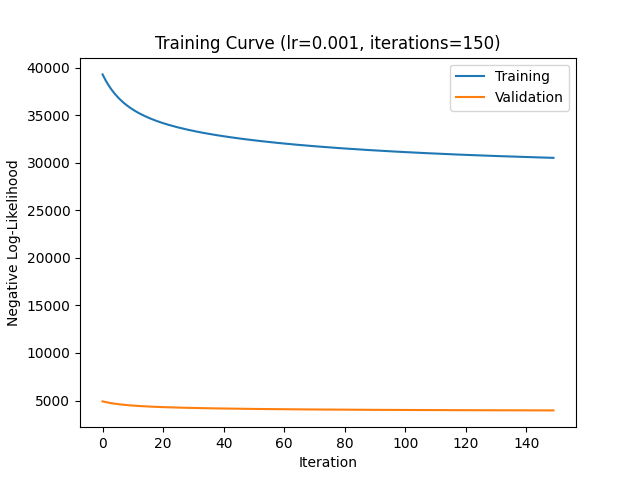
\includegraphics[width=0.7\textwidth]{irt_training_curve.png}
    \caption{Training and validation negative log-likelihood vs. iteration ($\eta=0.001$, 150 iterations).}
    \label{fig:irt_training}
\end{figure}

\subsubsection*{(c) Final accuracy}
With the selected hyperparameters, the final validation accuracy was $\mathbf{70.79\%}$ (matching the boxed entry in Table~\ref{tab:irt_tune}) and the final test accuracy was $\mathbf{70.28\%}$. The test accuracy is slightly lower than the $\eta=0.01$ setting we had used previously ($70.63\%$ validation, $70.79\%$ test), even though the new hyperparameters were chosen for higher validation accuracy. This is expected: the validation and test sets are different samples, so a small ($<1\%$) hyperparameter-driven improvement on one does not guarantee an identical improvement on the other.

\subsubsection*{(d) Probability curves}
Figure~\ref{fig:irt_prob} shows the probability of a correct response, $p(c_{ij}=1)$, as a function of student ability $\theta$, for three questions of varying difficulty.

\begin{figure}[H]
    \centering
    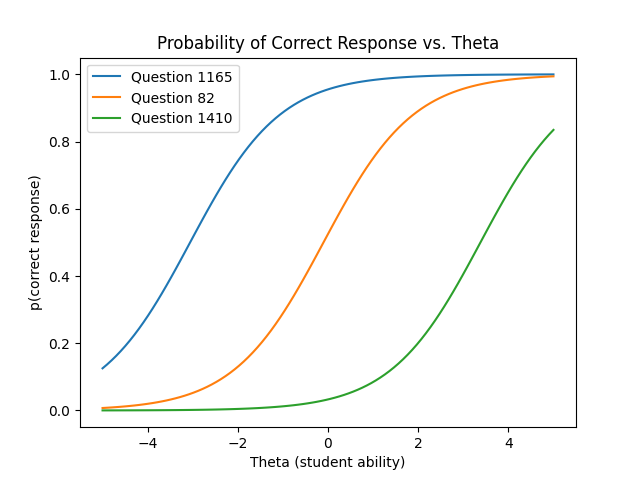
\includegraphics[width=0.7\textwidth]{irt_probability_curves.png}
    \caption{Probability of correct response vs. $\theta$ for three questions of varying difficulty.}
    \label{fig:irt_prob}
\end{figure}

All three curves follow the same sigmoid shape but are horizontally shifted according to each question's difficulty parameter $\beta_j$. The curve for Question 1165 is shifted furthest left, indicating the lowest difficulty: even students with below-average ability have a high probability of answering correctly. Conversely, Question 1410 is shifted right, requiring a much higher ability level before the probability of a correct response becomes non-negligible. Question 82 lies in between. The consistent sigmoid shape across all three reflects the core assumption of the one-parameter IRT model: correctness probability depends only on the gap $\theta_i - \beta_j$, so difficulty acts purely as a horizontal shift of the same underlying logistic curve.
 
% ============================================================
\subsection*{3. Matrix Factorization / Neural Network}
% --------------------------------------------------
% Part (a)
% --------------------------------------------------
\subsubsection*{(a)}

There are several key differences between ALS and neural networks:
\begin{itemize}
    \item \textbf{Model expressiveness.} 
    ALS assumes the prediction is simply the dot product of two vectors, $C_{nm} \approx \mathbf{u}_n^\top \mathbf{z}_m$, which is a bilinear model and can only capture linear relationships. The neural network introduced the sigmoid non-linearity between the two weight layers, so it can model more complex, non-linear relationships between student ability and question difficulty.

    \item \textbf{Parameter structure.} 
    In matrix factorization trained via ALS, each student has its own latent vector $\mathbf{u}_n$ and each question has its own latent vector $\mathbf{z}_m$; these parameters are learned directly, and their number grows linearly with the number of students and questions. In the neural network, all students share the same set of weights $\mathbf{W}^{(1)}$, $\mathbf{W}^{(2)}$  and biases $\mathbf{b}^{(1)}$, $\mathbf{b}^{(2)}$. A student's ``representation'' is not a freely learned parameter but is instead computed by passing that student's raw answer vector through the network. Consequently, the number of parameters depends only on the number of questions and the chosen latent dimension, and does not grow with the number of students.

    \item \textbf{Optimization procedure.}
    ALS alternates between fixing $\mathbf{Z}$ and updating $\mathbf{U}$, then fixing $\mathbf{U}$ and updating $\mathbf{Z}$, repeating this process even when implemented with SGD. The neural network is trained end-to-end: all parameters ($\mathbf{W}^{(1)}$, $\mathbf{W}^{(2)}$, $\mathbf{b}^{(1)}$, $\mathbf{b}^{(2)}$) are updated jointly in a single backward pass, with no alternating step.

    \item \textbf{Gradient computation.}
    In ALS, we must manually derive the gradient of the loss with respect to $\mathbf{u}_n$ and $\mathbf{z}_m$ and hand-code the update rule. In the neural network, gradients are computed automatically via PyTorch's autograd. The only thing we need to define is the forward pass, and backpropagation is handled by the framework.
\end{itemize}

% --------------------------------------------------
% Part (b)
% --------------------------------------------------
\subsubsection*{(b)}

The forward function defines a single pass of the autoencoder: it takes a student's answer vector as input, compresses it, and then reconstructs it back to its original size.

\textbf{Step 1 — Encoding.} self.g(inputs) applies a linear transformation that maps the 1774-dimensional input down to a k-dimensional vector. Wrapping it with torch.sigmoid squashes every value into the range [0, 1], producing the hidden representation hidden. This step compresses the student's full answer pattern into a smaller latent representation of size k.

\textbf{Step 2 — Decoding.} self.h(hidden) applies a second linear transformation that maps the k-dimensional hidden vector back up to 1774 dimensions. Wrapping it with torch.sigmoid again squashes each output into [0, 1], giving the final output out which is interpreted as the model's predicted probability that the student answers the corresponding question correctly. 

% --------------------------------------------------
% Part (c)
% --------------------------------------------------
\subsubsection*{(c)}

In addition to $k$, we jointly tuned the learning rate $\text{lr} \in \{0.001, 0.003, 0.01, 0.03, 0.1\}$ and the number of training epochs $\in \{10, 20, 30, 40, 50\}$ (125 combinations total). Table~\ref{tab:nn-k-lr} reports, for each $(k, \text{lr})$ pair, the best validation accuracy achieved over the 5 epoch settings.

\begin{table}[H]
\centering
\caption{Validation accuracy for each $(k, \text{lr})$ pair, best over epoch $\in \{10,20,30,40,50\}$.}
\label{tab:nn-k-lr}
\begin{tabular}{c|ccccc}
\toprule
$k$ \textbackslash\ lr & 0.001 & 0.003 & 0.01 & \textbf{0.03} & 0.1 \\
\midrule
\textbf{10} & 0.6129 & 0.6377 & 0.6822 & \textbf{0.6922} & 0.6856 \\
50 & 0.6307 & 0.6660 & 0.6897 & 0.6813 & 0.6739 \\
100 & 0.6349 & 0.6671 & 0.6819 & 0.6816 & 0.6715 \\
200 & 0.6362 & 0.6719 & 0.6833 & 0.6722 & 0.6624 \\
500 & 0.6359 & 0.6739 & 0.6744 & 0.6668 & 0.6644 \\
\bottomrule
\end{tabular}
\end{table}

The best combination is $k^*=10$, $\text{lr}^*=0.03$ (achieved after $20$ training epochs), giving a validation accuracy of $0.6922$.
% --------------------------------------------------
% Part (d)
% --------------------------------------------------
\subsubsection*{(d)}

\begin{figure}[H]
    \centering
    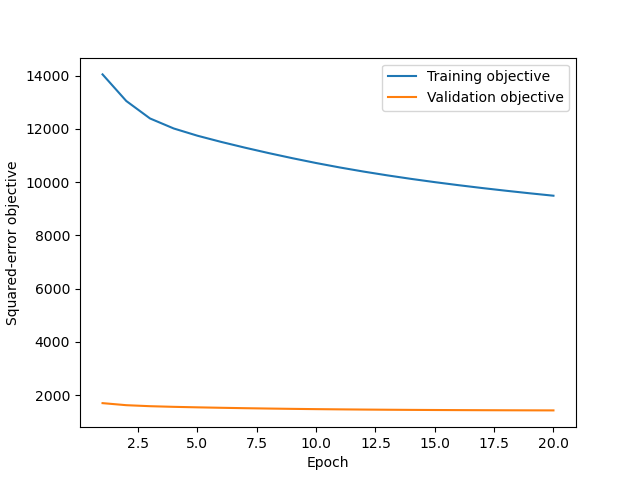
\includegraphics[width=0.5\linewidth]{nn_objective_curve.png}
    \caption{Neural network training/validation objective curve}
\end{figure}

Final test accuracy (k*=10, lr*=0.03, 20 epochs, $\lambda=0$): \textbf{0.6856}

% --------------------------------------------------
% Part (e)
% --------------------------------------------------
\subsubsection*{(e)}

Using $\lambda^* = 0.001$ (selected via validation accuracy, tested over $\lambda \in \{0.0, 0.001, 0.01, 0.1, 1.0\}$ with $k^*=10$ and $\text{lr}^*=0.03$ fixed), the final model achieves:
\begin{itemize}
    \item Validation accuracy: $0.6820$
    \item Test accuracy: $0.6760$
\end{itemize}
Compared to the unregularized model ($\lambda = 0$) with the same $k^*$ and $\text{lr}^*$, which achieved a test accuracy of $0.6856$, the regularized model performs slightly worse (a difference of about $0.0096$). We therefore conclude that adding the $L_2$ regularization penalty does not improve generalization performance in this setting, and may in fact slightly hurt it. This is likely because the autoencoder's hidden dimension $k^*=10$ is already very small relative to the number of questions, which acts as a strong implicit regularizer by limiting the model's capacity to overfit; an explicit weight penalty on top of this therefore offers no additional benefit and can instead constrain the model away from its unregularized optimum.
% ============================================================
\subsection*{4. Ensemble}

We bootstrap the training set 3 times, sampling with replacement each time, and train one base model per resample. For kNN and the autoencoder, the resample is stored as a matrix; for IRT, it is kept as a list of observations so that duplicated pairs are correctly double-counted during gradient ascent. Each trained base model outputs a predicted probability of "correct" for every $(i,j)$ pair in the validation and test sets; we average the 3 probabilities and threshold at $0.5$ to get the ensemble's prediction. Bagging in this way reduces variance since each base model sees a different resample of the data, their errors are only partially correlated.

\begin{table}[H]
\centering
\caption{Validation and test accuracy of each base model and of the bagged ensemble.}
\begin{tabular}{lcc}
\toprule
Model & Validation accuracy & Test accuracy \\
\midrule
kNN alone & 0.6544 & 0.6610 \\
IRT alone & 0.6983 & 0.6938 \\
NN alone & 0.6509 & 0.6497 \\
\textbf{Ensemble (average)} & \textbf{0.6820} & \textbf{0.6777} \\
\bottomrule
\end{tabular}
\end{table}

The ensemble's accuracy sits between the strongest base model (IRT) and the two weaker ones (kNN, NN), rather than exceeding all three. Though the ensemble clearly outperforms the two weaker base models individually, with only 3 base learners of unequal quality, unweighted averaging cannot fully recover the accuracy of the single best model.

\clearpage
\section*{Part B}
 
\subsection*{1. Formal Description}

\textbf{Motivation.} Part A's user- and item-based KNN impute a pair $(i,j)$ from only the $k$ nearest rows/columns under a NaN-aware Euclidean distance. When a student or question has few observations, this neighbourhood is small and the imputed probability is noisy: KNN is low-bias but high-variance in sparse regions of $C$. We reduce this variance by blending KNN with a much lower-variance, higher-bias estimate: the simple average of all training observations for that student or question.

\textbf{Base predictors.} Let $C \in \{0,1,\mathrm{NaN}\}^{N \times M}$ be the training matrix ($N=542$ students, $M=1774$ questions), $O$ the observed pairs, and $\hat{c}^{\text{user}}_{ij}, \hat{c}^{\text{item}}_{ij} \in [0,1]$ the Part A user- ($k{=}11$) and item- ($k{=}21$) KNN probabilities. Define two correctness priors from the training data, each falling back to the global rate $\bar{c}$ if the row/column has no observations:
\[
\pi^{q}_j = \frac{\sum_{i : (i,j) \in O} c_{ij}}{|\{i : (i,j) \in O\}|}, \qquad
\pi^{s}_i = \frac{\sum_{j : (i,j) \in O} c_{ij}}{|\{j : (i,j) \in O\}|}.
\]

\textbf{Hybrid model.} Given weights $\alpha, \beta, \gamma \in [0,1]$ and threshold $\tau$:
\[
p^{\text{knn}}_{ij}(\alpha) = \alpha\, \hat{c}^{\text{user}}_{ij} + (1-\alpha)\, \hat{c}^{\text{item}}_{ij}, \qquad
p^{\text{prior}}_{ij}(\beta) = \beta\, \pi^{q}_j + (1-\beta)\, \pi^{s}_i,
\]
\[
p_{ij}(\alpha,\beta,\gamma) = \gamma\, p^{\text{knn}}_{ij}(\alpha) + (1-\gamma)\, p^{\text{prior}}_{ij}(\beta), \qquad
\hat{c}_{ij} = \mathbb{1}[\,p_{ij} \geq \tau\,].
\]
This strictly generalizes Part A: $\gamma{=}1,\alpha{=}1$ recovers user-based KNN alone, and $\gamma{=}1,\alpha{=}0$ recovers item-based KNN alone.

\textbf{Hyperparameter selection.} $(\alpha,\beta,\gamma,\tau)$ and the base KNN configurations ($k$, uniform/distance weighting) are chosen by grid search to maximize \emph{validation} accuracy (Algorithm~\ref{alg:tuning}); the test set is touched only once, at the end.

\begin{algorithm}[H]
\caption{Validation-selected hybrid tuning}
\label{alg:tuning}
\begin{algorithmic}[1]
\STATE Fit every candidate user-/item-KNN config (Part A baseline + distance-weighted, $k \in \{5,\dots,50\}$); cache validation predictions.
\STATE Compute $\pi^{q}_j, \pi^{s}_i$ from $C$.
\STATE For every combination of configs and $(\alpha,\beta,\gamma,\tau)$: compute $p_{ij}$, $\hat c_{ij}$, and validation accuracy; keep the best.
\STATE Refit the selected configs, evaluate once on the test set.
\end{algorithmic}
\end{algorithm}

\textbf{Why this should help.} The hybrid convex-combines a low-bias/high-variance predictor ($p^{\text{knn}}$) with a high-bias/low-variance one ($p^{\text{prior}}$). Whenever the two make partially independent errors -- expected in sparse rows/columns, where KNN is unreliable but the priors' aggregates are not -- the combination has strictly lower expected squared error than either endpoint for some interior $\gamma$. Section 3 tests this directly, including which prior actually drives the improvement.

\subsection*{2. Figure or Diagram}

Figure~\ref{fig:partb_schematic} illustrates the overall structure of the Part B hybrid predictor described in Section 1.

\begin{figure}[H]
\centering
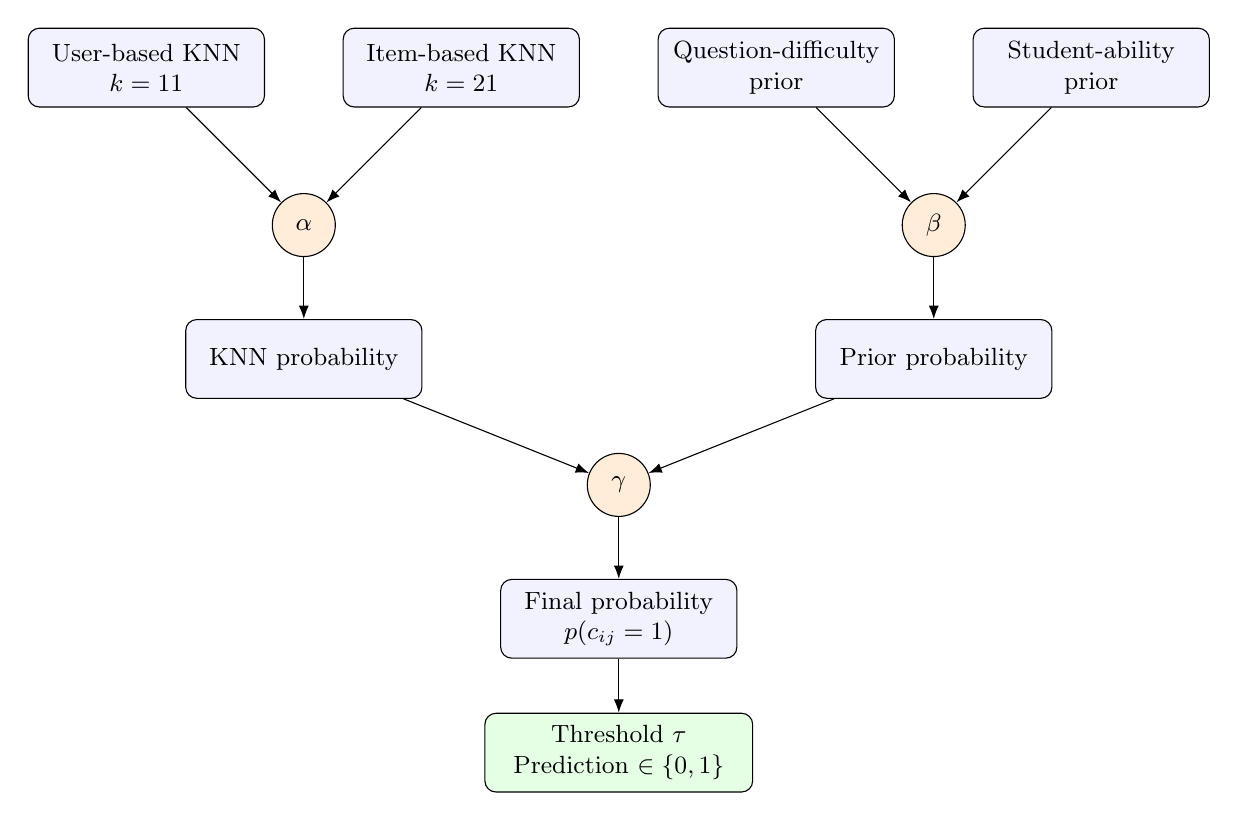
\begin{tikzpicture}[
    >=Latex,
    box/.style={draw, rounded corners, align=center, minimum height=1cm, minimum width=3cm, fill=blue!5, font=\small},
    combine/.style={draw, circle, minimum size=0.8cm, fill=orange!15, font=\small},
    final/.style={draw, rounded corners, align=center, minimum height=1cm, minimum width=3.4cm, fill=green!10, font=\small}
]

\node[box] (usernn) at (0, 6) {User-based KNN\\$k=11$};
\node[box] (itemnn) at (4, 6) {Item-based KNN\\$k=21$};
\node[box] (qprior) at (8, 6) {Question-difficulty\\prior};
\node[box] (sprior) at (12, 6) {Student-ability\\prior};

\node[combine] (alpha) at (2, 4) {$\alpha$};
\node[combine] (beta) at (10, 4) {$\beta$};

\node[box] (knnprob) at (2, 2.3) {KNN probability};
\node[box] (priorprob) at (10, 2.3) {Prior probability};

\node[combine] (gamma) at (6, 0.7) {$\gamma$};

\node[box] (finalprob) at (6, -1) {Final probability\\$p(c_{ij}=1)$};

\node[final] (threshold) at (6, -2.7) {Threshold $\tau$\\Prediction $\in \{0,1\}$};

\draw[->] (usernn) -- (alpha);
\draw[->] (itemnn) -- (alpha);
\draw[->] (qprior) -- (beta);
\draw[->] (sprior) -- (beta);
\draw[->] (alpha) -- (knnprob);
\draw[->] (beta) -- (priorprob);
\draw[->] (knnprob) -- (gamma);
\draw[->] (priorprob) -- (gamma);
\draw[->] (gamma) -- (finalprob);
\draw[->] (finalprob) -- (threshold);

\end{tikzpicture}
\caption{Schematic of the Part B hybrid predictor. User- and item-based KNN outputs are blended by $\alpha$; the question-difficulty and student-ability priors are blended by $\beta$; the resulting KNN and prior probabilities are blended by $\gamma$ and thresholded at $\tau$ to produce the final prediction.}
\label{fig:partb_schematic}
\end{figure}
\subsection*{3. Comparison or Demonstration}

\subsubsection*{Accuracy comparison}

Table~\ref{tab:partb_results} reports validation/test accuracy for the Part A baselines and each stage of the hybrid, all selected using validation accuracy only (Figure~\ref{fig:partb_comparison} shows the same visually).

\begin{table}[H]
    \centering
    \begin{tabular}{lcc}
        \toprule
        Model & Validation Accuracy & Test Accuracy \\
        \midrule
        Part A user KNN ($k=11$)
        & $68.97\%$ & $68.47\%$ \\

        Part A item KNN ($k=21$)
        & $69.16\%$ & $68.28\%$ \\

        Best tuned user KNN
        & $68.97\%$ & $68.47\%$ \\

        Best tuned item KNN
        & $69.16\%$ & $68.28\%$ \\

        50--50 user/item hybrid
        & $70.41\%$ & $69.63\%$ \\

        Hybrid + question-difficulty prior only
        & $70.49\%$ & $70.17\%$ \\

        Hybrid + student-ability prior only
        & $70.90\%$ & $70.03\%$ \\

        \textbf{Final hybrid (both priors, tuned)}
        & \textbf{$71.15\%$} & \textbf{$70.79\%$} \\
        \bottomrule
    \end{tabular}
    \caption{Comparison of Part A KNN baselines against the Part B
    hybrid and its ablations.}
    \label{tab:partb_results}
\end{table}

\begin{figure}[H]
    \centering
    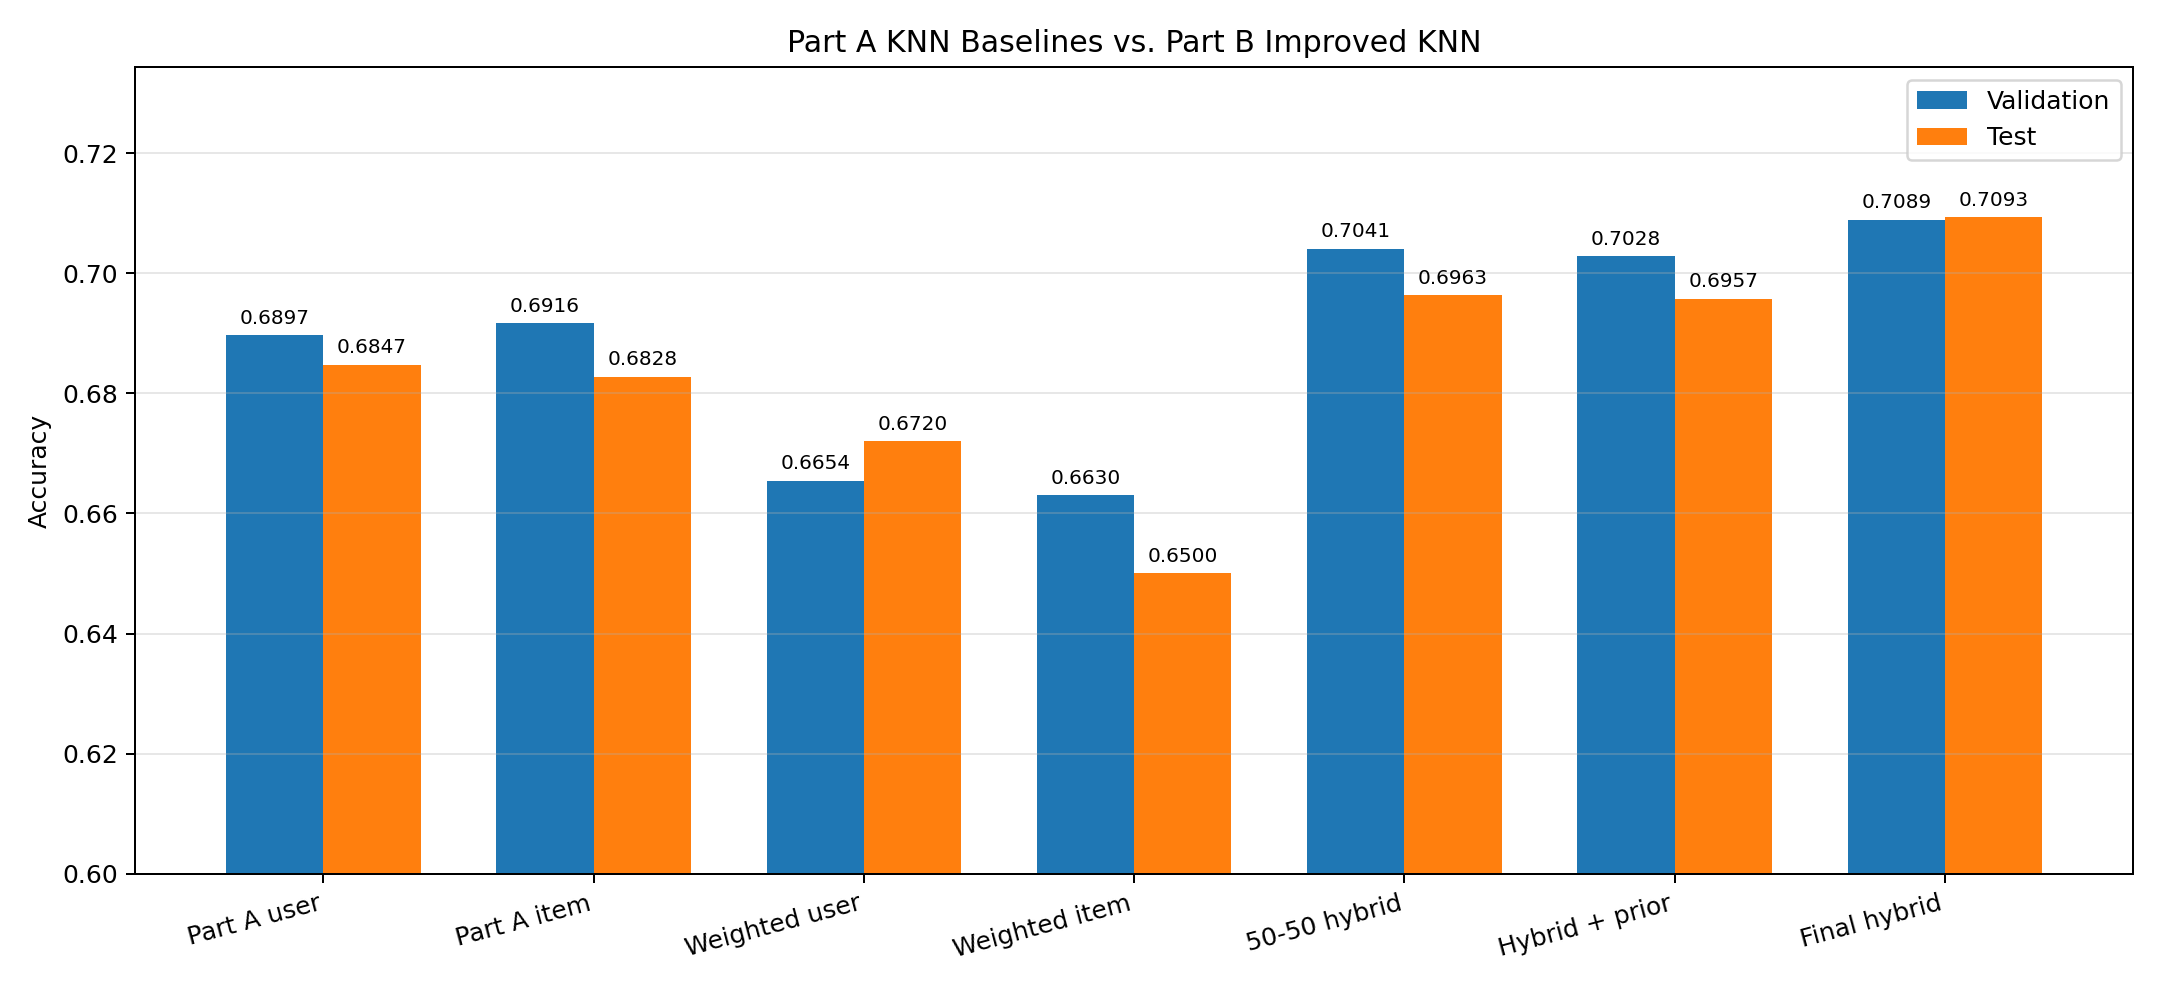
\includegraphics[width=0.95\textwidth]{partb_knn_comparison.png}
    \caption{Validation and test accuracy for the Part A baselines and
    each stage of the Part B hybrid.}
    \label{fig:partb_comparison}
\end{figure}

The final hybrid improves test accuracy by roughly $2.3$ points over the stronger Part A baseline ($68.47\% \to 70.79\%$) and by $1.2$ points over a naive unweighted user/item average ($69.63\% \to 70.79\%$), so the gain is not simply from averaging two noisy predictors.

\subsubsection*{Disentangling the source of the improvement}

We hypothesized that KNN is limited by sparsity: individual students/questions have few observations, so imputed probabilities are noisy. Two changes were expected to help: (i) combining user- and item-based KNN, and (ii) backing off toward low-variance correctness priors. Two experiments isolate which actually helps.

\textbf{Experiment 1 -- which prior helps?} Adding only the question prior raises validation accuracy from $70.41\%$ to $70.49\%$ ($69.63\%\to70.17\%$ test); the student prior alone raises it further to $70.90\%$ ($70.03\%$ test). Combining both equally ($\beta=0.50$) beats either alone, reaching $71.15\%$ validation / $70.79\%$ test. This matches the intuition that per-student and per-question correctness rates carry independent signal beyond what KNN captures, so mixing both priors reduces variance more than either alone.

\textbf{Experiment 2 -- priors, or just a larger search?} The independently best-tuned user/item KNN models score no higher than the Part A baselines ($68.97\%/68.47\%$ and $69.16\%/68.28\%$), while combining them reaches $70.41\%$ validation and adding both priors reaches $71.15\%$. So the improvement is attributable to combining the priors and the two KNN sources, not to a larger KNN hyperparameter search.

Figure~\ref{fig:partb_tuning} shows validation sensitivity to $\beta$ and to $(\gamma,\tau)$ at the selected configuration ($\alpha=0.50$, $\beta=0.50$, $\gamma=0.70$, $\tau=0.55$, $71.15\%$ validation). Expanding all four weights, the final probability places $35\%$/$35\%$ on user/item KNN and $15\%$/$15\%$ on the question/student priors. The selected $(\gamma,\tau)$ lies at the edge of the searched grid, suggesting a wider search could help further (see Limitations).

\begin{figure}[H]
    \centering
    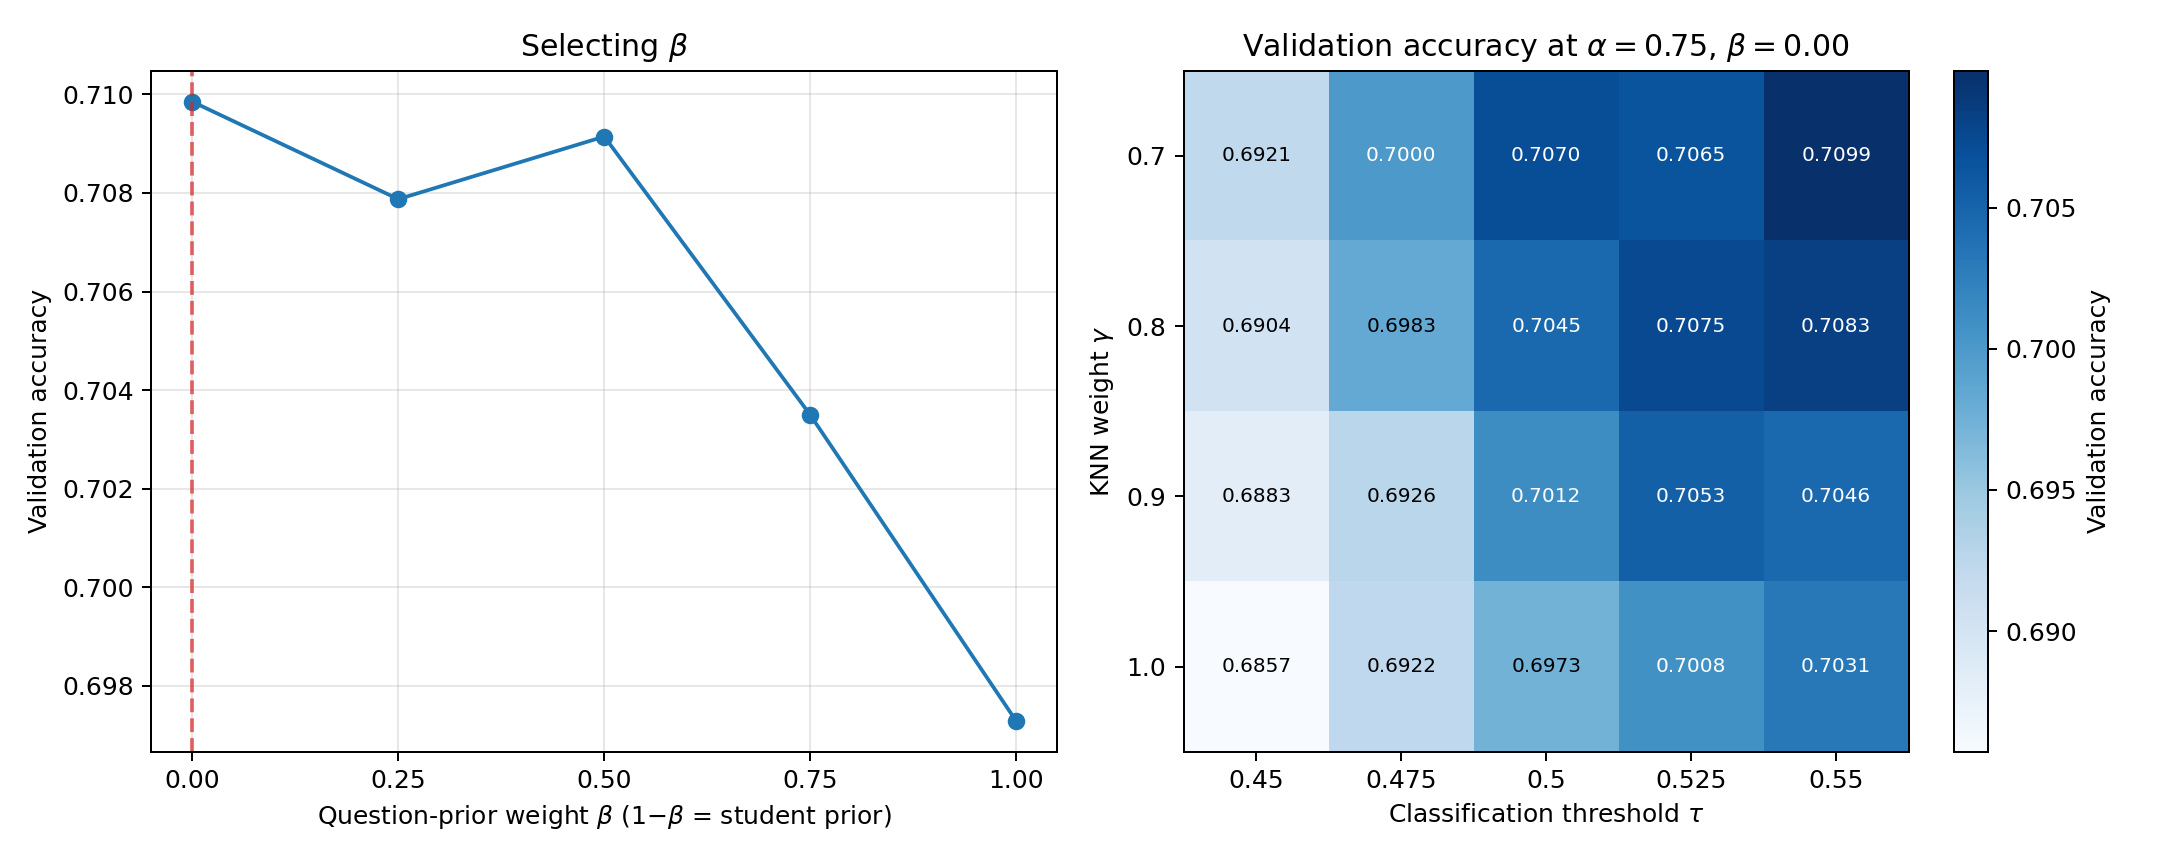
\includegraphics[width=0.95\textwidth]{partb_knn_tuning.png}
    \caption{Validation accuracy as a function of the prior-blend
    weight $\beta$ (left), and as a function of the KNN-vs-prior weight
    $\gamma$ and threshold $\tau$ at the selected
    $\alpha=0.50$ and $\beta=0.50$ (right).}
    \label{fig:partb_tuning}
\end{figure}

\subsection*{4. Limitations}

\textbf{Sparsity is only partially addressed.} Each prior is still just one scalar per student/question, and falls back to the global average when observations are scarce. A true cold-start student or question with zero training observations would leave both the KNN predictors and the priors with little useful information.

\textbf{Heuristic rather than principled combination.} Unlike IRT, which derives $p(c_{ij}=1)$ from an explicit probabilistic model, our hybrid combines KNN outputs and priors via validation-selected linear weights $(\alpha,\beta,\gamma,\tau)$ with no principled rule for how much weight each component should get. These weights are dataset-dependent and would likely need re-tuning for a different response matrix or student-to-question ratio.

\textbf{Sensitivity to hyperparameter selection.} The validation set ($\sim$1500 rows) may not reliably distinguish near-tied configurations, and the selected $(\gamma,\tau)$ lies at the edge of the searched grid rather than an interior maximum -- a wider, finer search might do better. We also observed, while re-running our own code on different machines, that the selected $(\alpha,\beta,\gamma,\tau)$ is not perfectly stable: small floating-point differences in the nearest-neighbour distance computation across library versions can change which near-tied grid point is picked. The reported test accuracy is therefore a point estimate; a different validation split, search range, or computing environment could select a slightly different configuration. Cross-validation or a larger held-out set would make selection more robust.

\textbf{Unused structure.} We did not use \texttt{question\_meta.csv} or \texttt{student\_meta.csv}. A hierarchical prior -- e.g. backing off a sparse question's difficulty to its subject's average rather than the global average -- is a natural extension, as is incorporating student metadata for students with limited response histories.
\end{document}
